%----------------------------------------------------------------------------------------
%	CHAPTER 5 // Eye Tracking Discussion and Evaluation
%----------------------------------------------------------------------------------------
\chapterimage{cover_4.png}
\chapter{Discussion and Evaluation} \index{Eye Tracking Discussion and Evaluation}

\section{Evaluation}\index{Evaluation}
In the previous chapters we discussed Starburst \cite{starburst}, Pupil \cite{pupil}, and MIRT eye tracking algorithms. Both Starburst and Pupil use infrared spectrum imaging. On the other hand MIRT is using visible spectrum imaging. Using visible spectrum is more complicated due to uncontrolled lighting conditions, which contain multiple specular and diffuse components. Capturing infrared images requires either using infrared cameras or using infrared lighting source with a traditional camera. For example \cite{scriptwear} describes  how to hack a traditional USB webcam to capture infrared images by removing the infrared filter and adding an infrared LED on camera chip. \bigskip

In MIRT we use visible spectrum which frees us from using special hardware. In visible spectrum images the corneal limbus (usually referred as limbus) is the strongest feature contour in the image, rather than the pupil which is the strongest feature contour when using infrared imaging. \bigskip

\begin{figure*}[!h]
\begin{dBox}
\centering
	\mbox{
		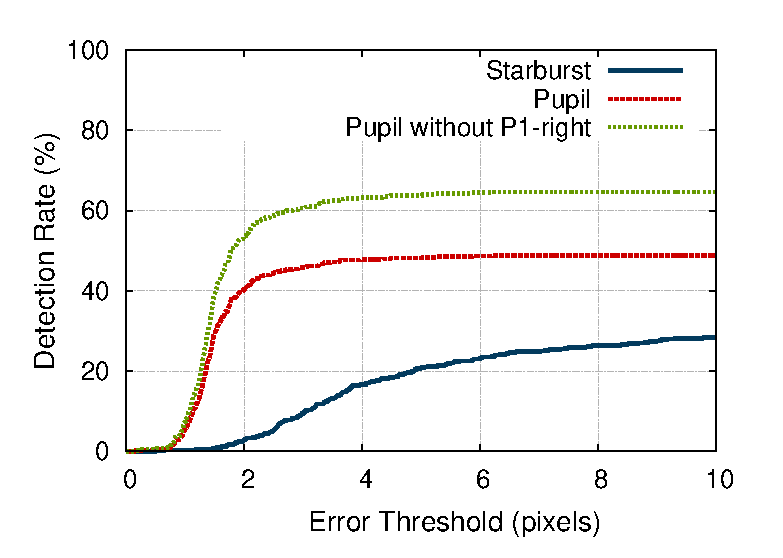
\includegraphics[width=\textwidth]{./Pictures/evaluation/error.eps}
	}
   \caption{Comparison of pupil detection rate between our implementation of Pupil algorithm and our implementation of Starburst algorithm using benchmark dataset by Swirski et al.\label{fig:our_eval} }   
\end{dBox}   
\end{figure*}

To evaluate our implementation of Starburst and Pupil we used the the benchmark dataset by Swirski et al. \cite{swirski}. Figure \ref{fig:our_eval} shows performance comparison between our implementation of Starburst described in chapter \ref{ch_starburst} and our implementation of Pupil algorithm \ref{ch_pupil}. As the figure indicates the performance of Starburst is relatively low compared to Pupil. The fall back in Starburst performance mainly results from the initial guess of the pupil center. A notable observation during the evaluation is that Starburst usually drops many frames until it detects the pupil, whenever the pupil is first is detected the detection rate in successive frames increase significantly. We tried to short circuit the Starburst initial estimate of pupil center (image center) with the actual pupil location I the first frame but the detection rate wasn't much affected. \bigskip

Moving to Pupil it can be clearly seen that Pupil overcomes Starburst. Pupil achieves about 48\% detection rate when evaluated using the complete dataset. If we exclude the dataset p1-right, that contains eye images recorded at the most extreme angles, the detection rate rise to 64\%. \bigskip

\begin{figure*}[!h]
\begin{dBox}
\centering
	\mbox{
		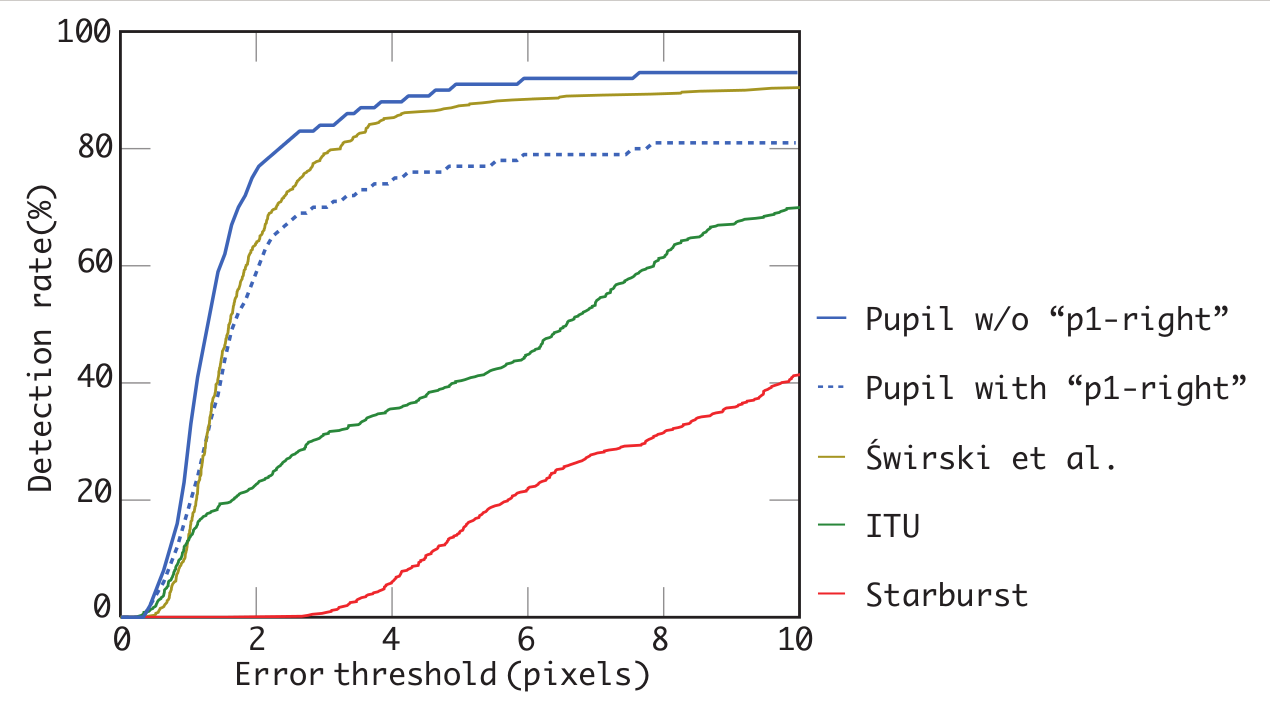
\includegraphics[width=\textwidth]{./Pictures/evaluation/comparison_pupil.png}
	}
   \caption{Comparison of pupil detection rate for Pupil’s algorithm, the stock algorithm proposed by Swirski et al., the ITU gaze tracker and Starburst. Figure from Pupil \cite{starburst} \label{fig:pupil_eval} }   
\end{dBox}   
\end{figure*}

Figure \ref{fig:pupil_eval} shows the evaluation on the same dataset mentioned in Pupil paper \cite{pupil} . This figure shows the performance difference between our implementation of Starburst and Pupil and actual implementations of both algorithms. Starburst we almost achieved the same performance level. On the other hand our implementation of pupil is about 20\% less accurate than the actual implementation.




\section{Headset Design and Hardware} \index{Headset Design and Hardware}
In our system we build a cheap (do it yourself - DIY) head mounded eye-tracker. Figure \ref{fig:headset} shows the prototype of our eye tracker. We used a traditional glasses frame after removing the lenses. Then we attached an internal laptop webcam to the frame. The webcam we used is a USB HP webcam. The chip comes with 2 integrated microphones, hence the camera chip has 6 pins while the USB has 4 wires. Correct pinout can be found at \cite{myblogpost}.



\begin{figure*}[!h]
\begin{dBox}
\centering
	\mbox{
		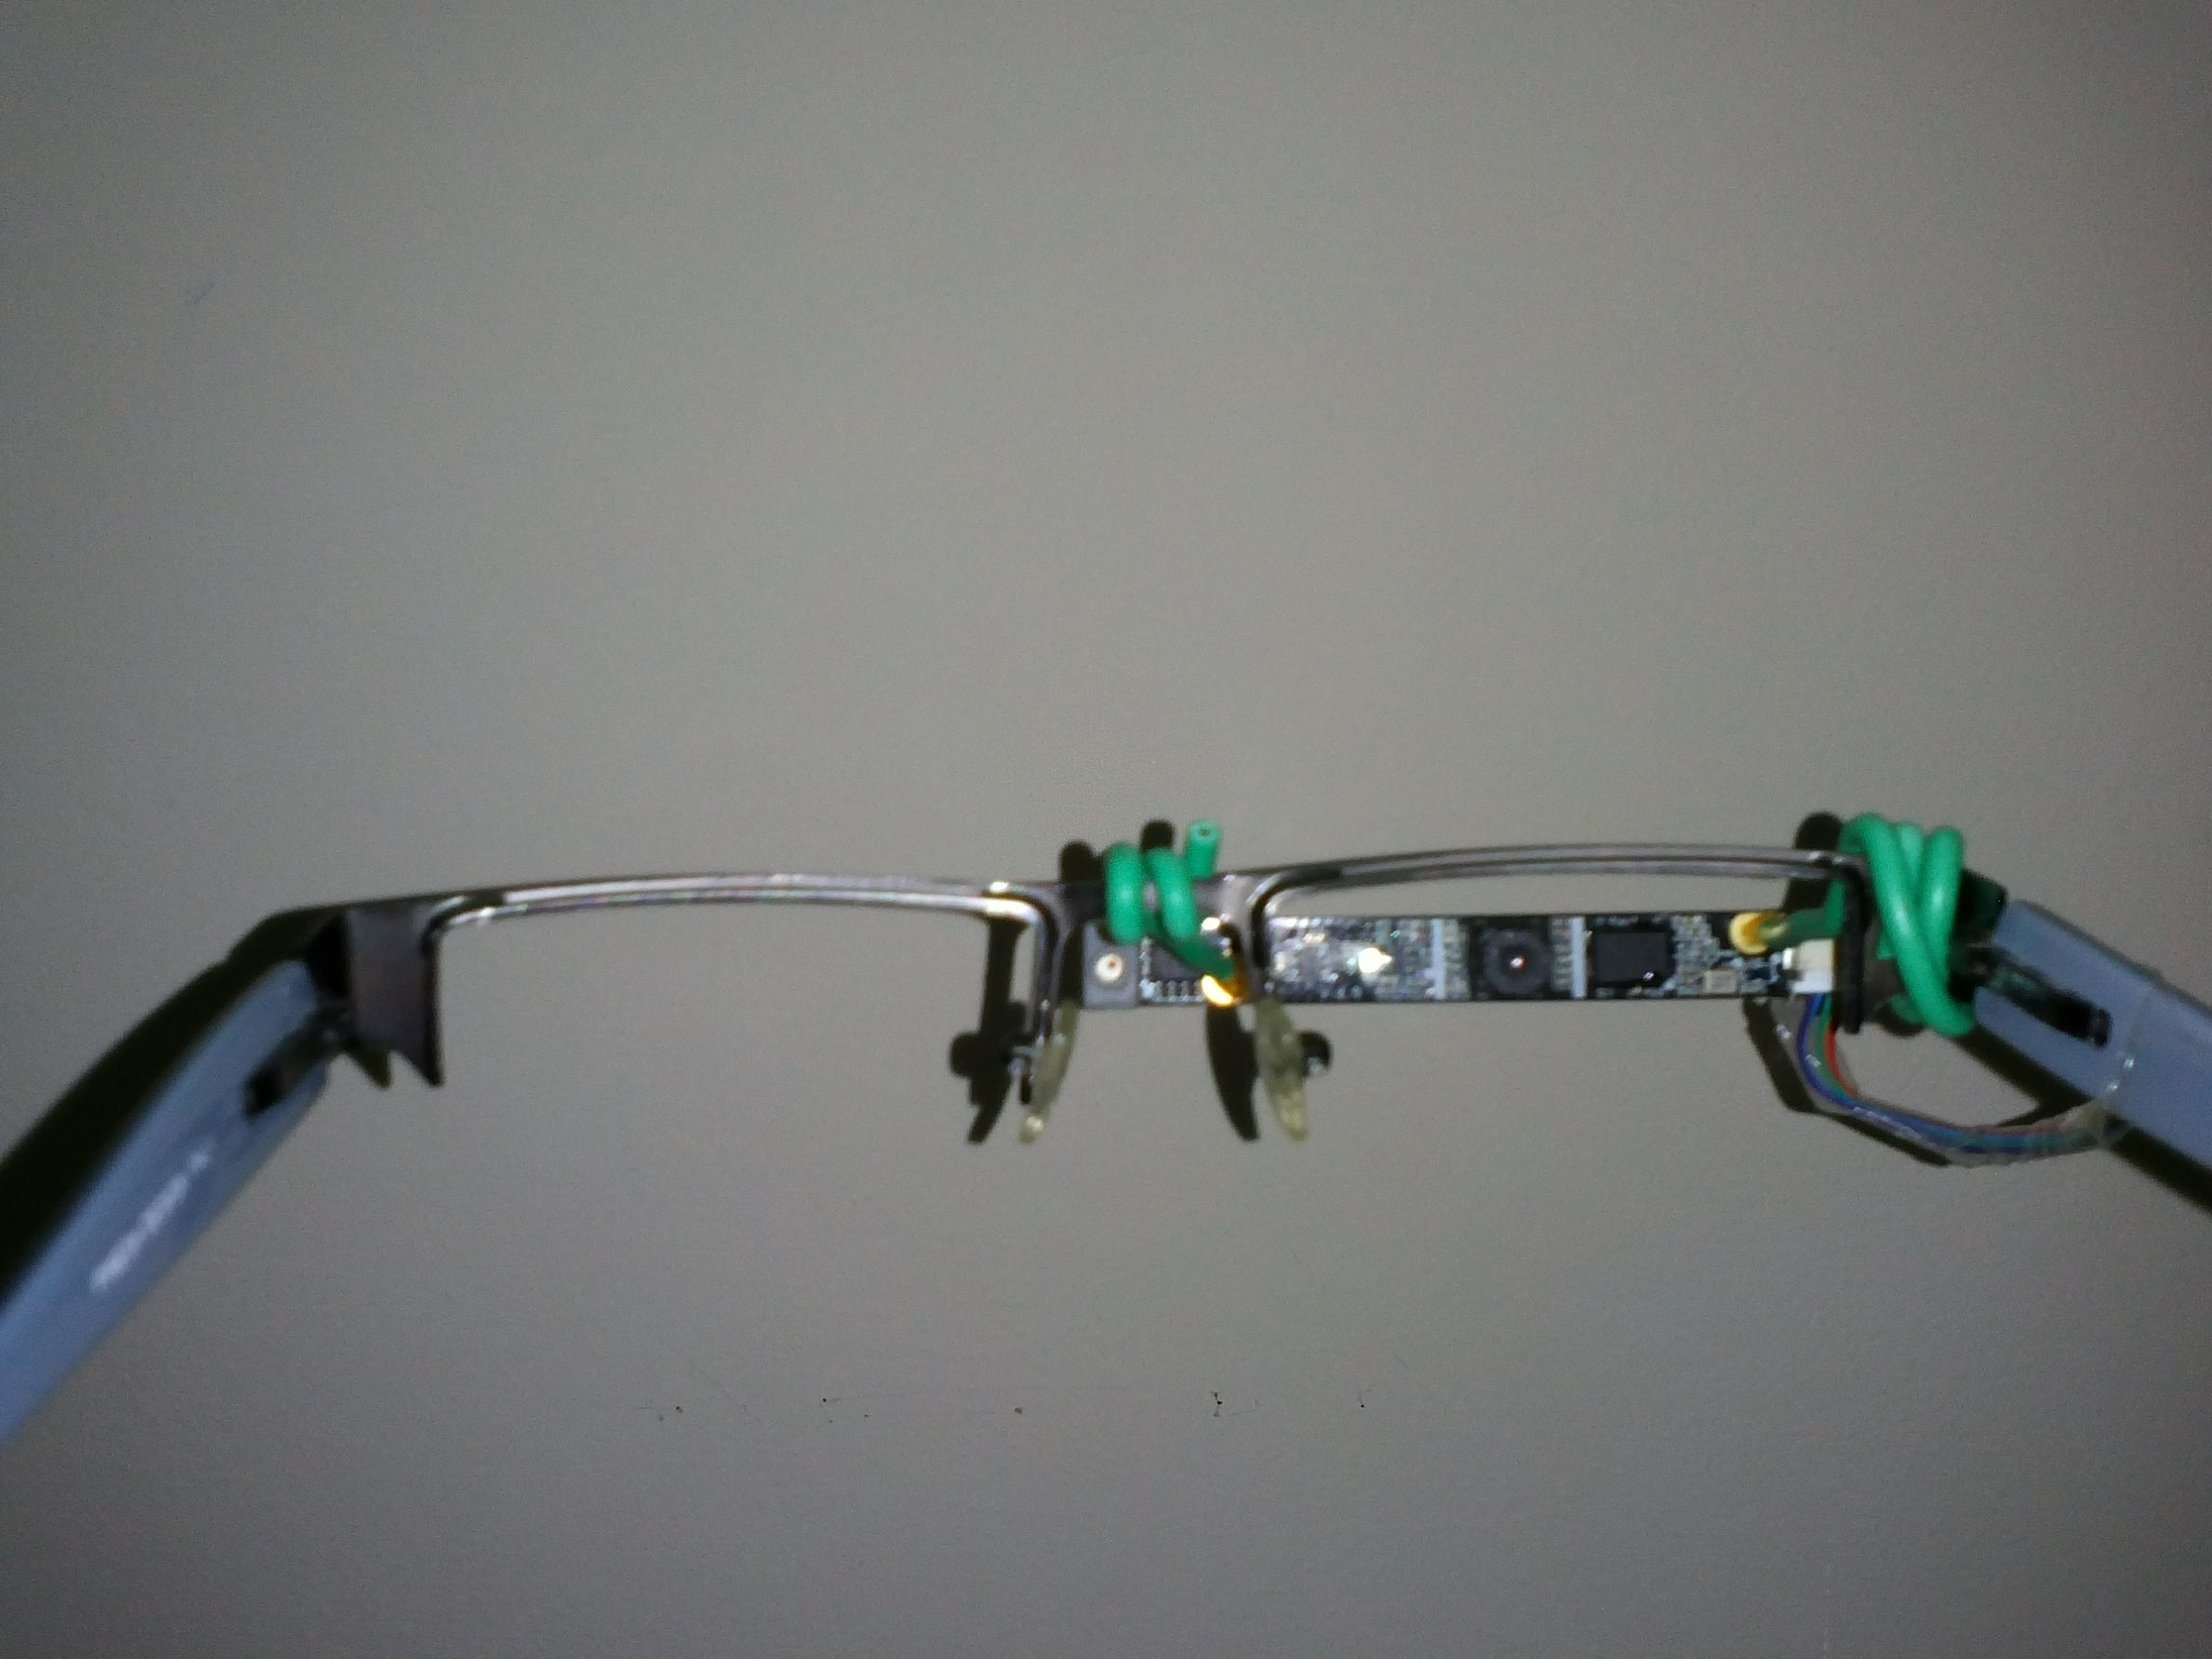
\includegraphics[width=.45\textwidth]{./Pictures/evaluation/cam_front.jpg}
		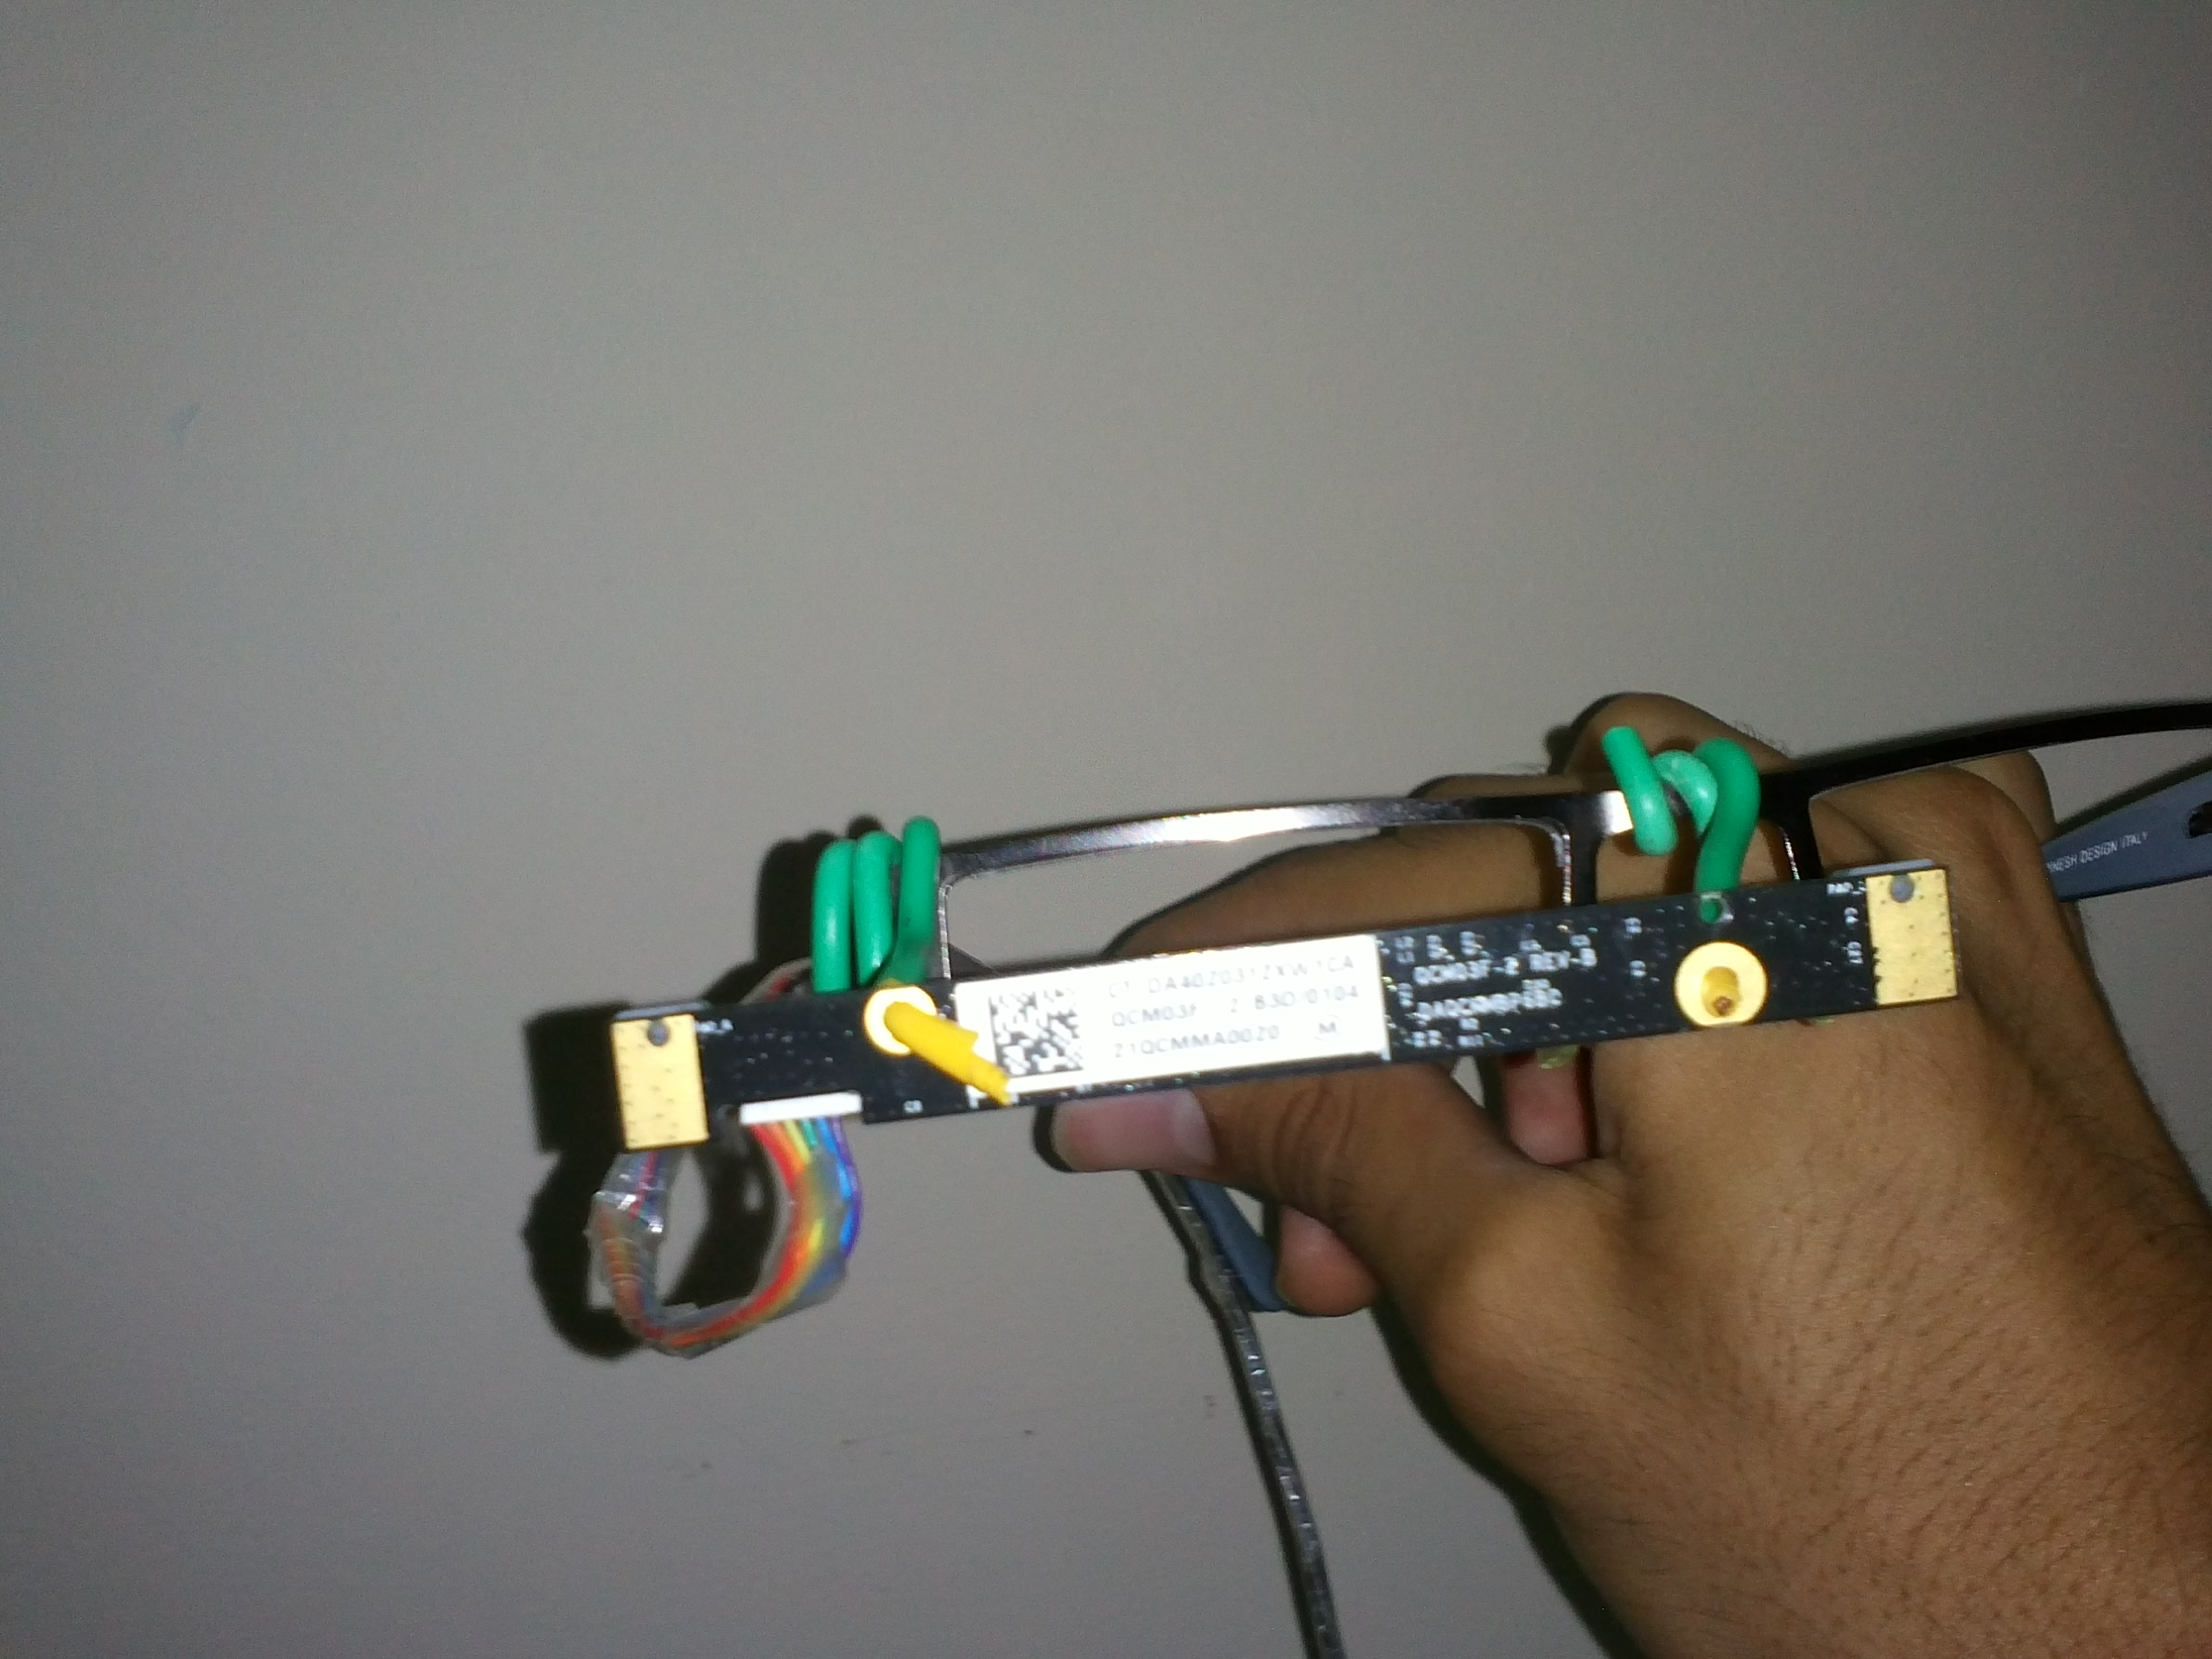
\includegraphics[width=.45\textwidth]{./Pictures/evaluation/cam_back.jpg}
	}
	\mbox{
		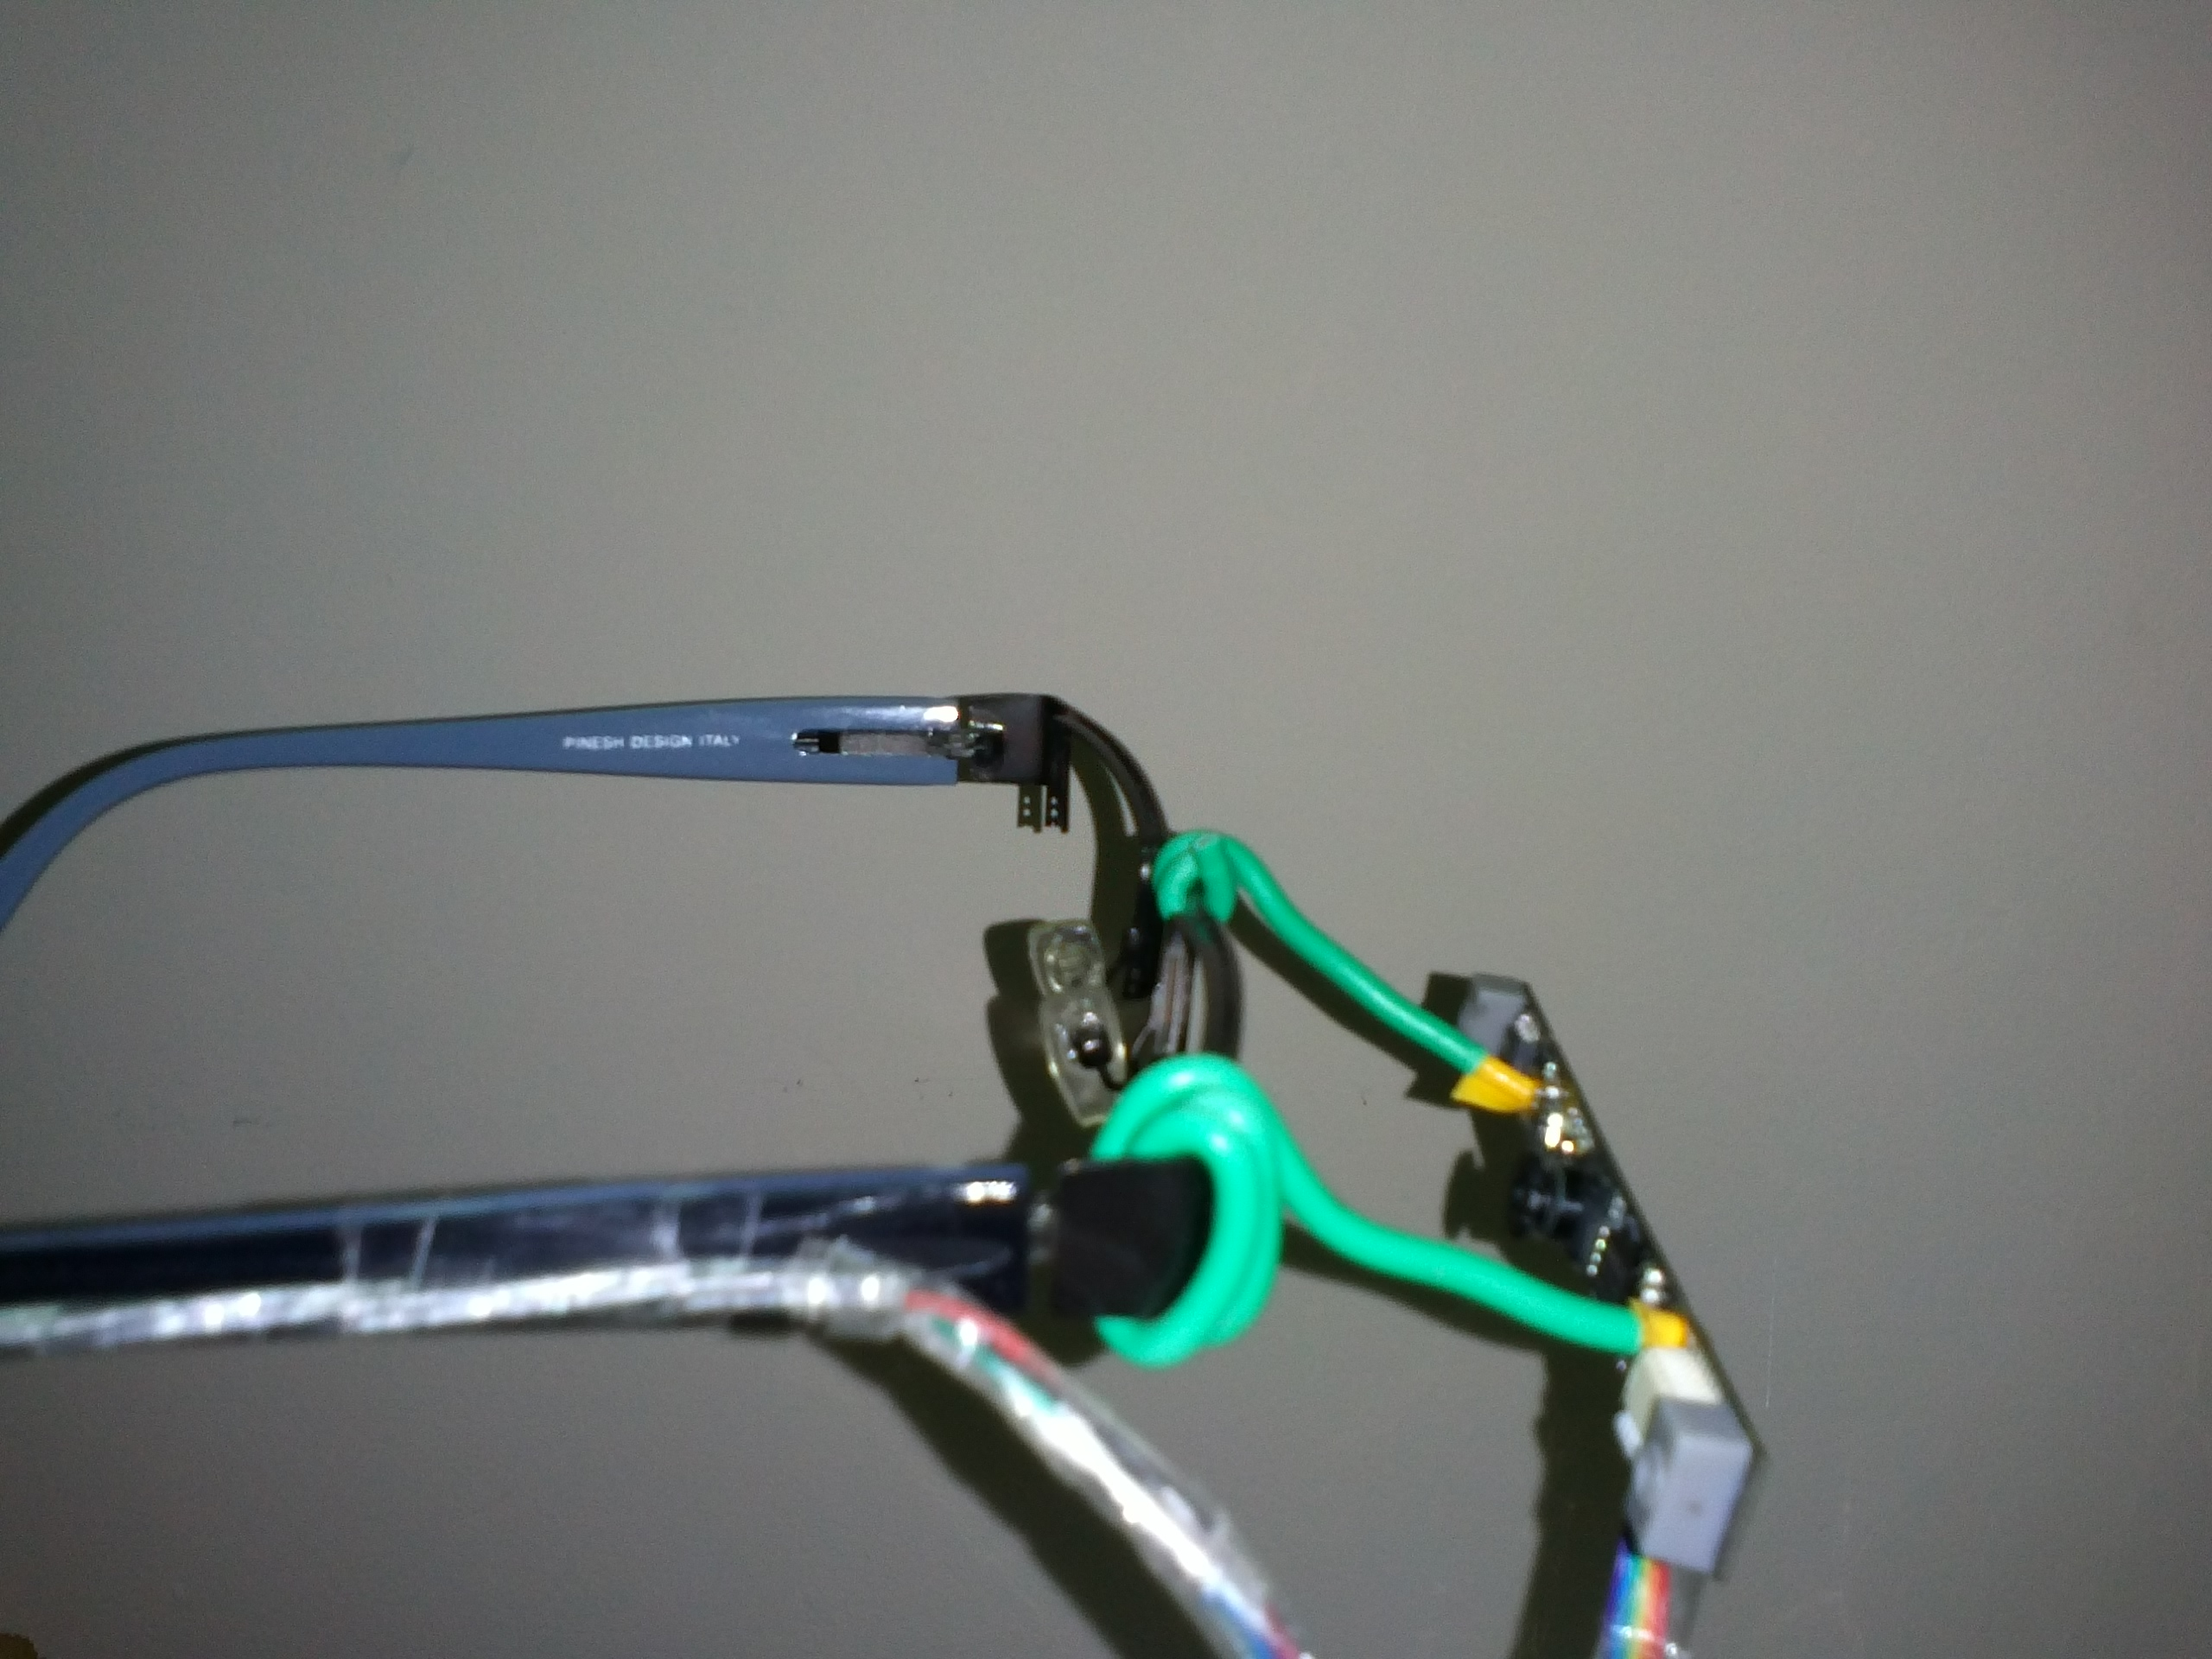
\includegraphics[width=.45\textwidth]{./Pictures/evaluation/cam_side.jpg}
		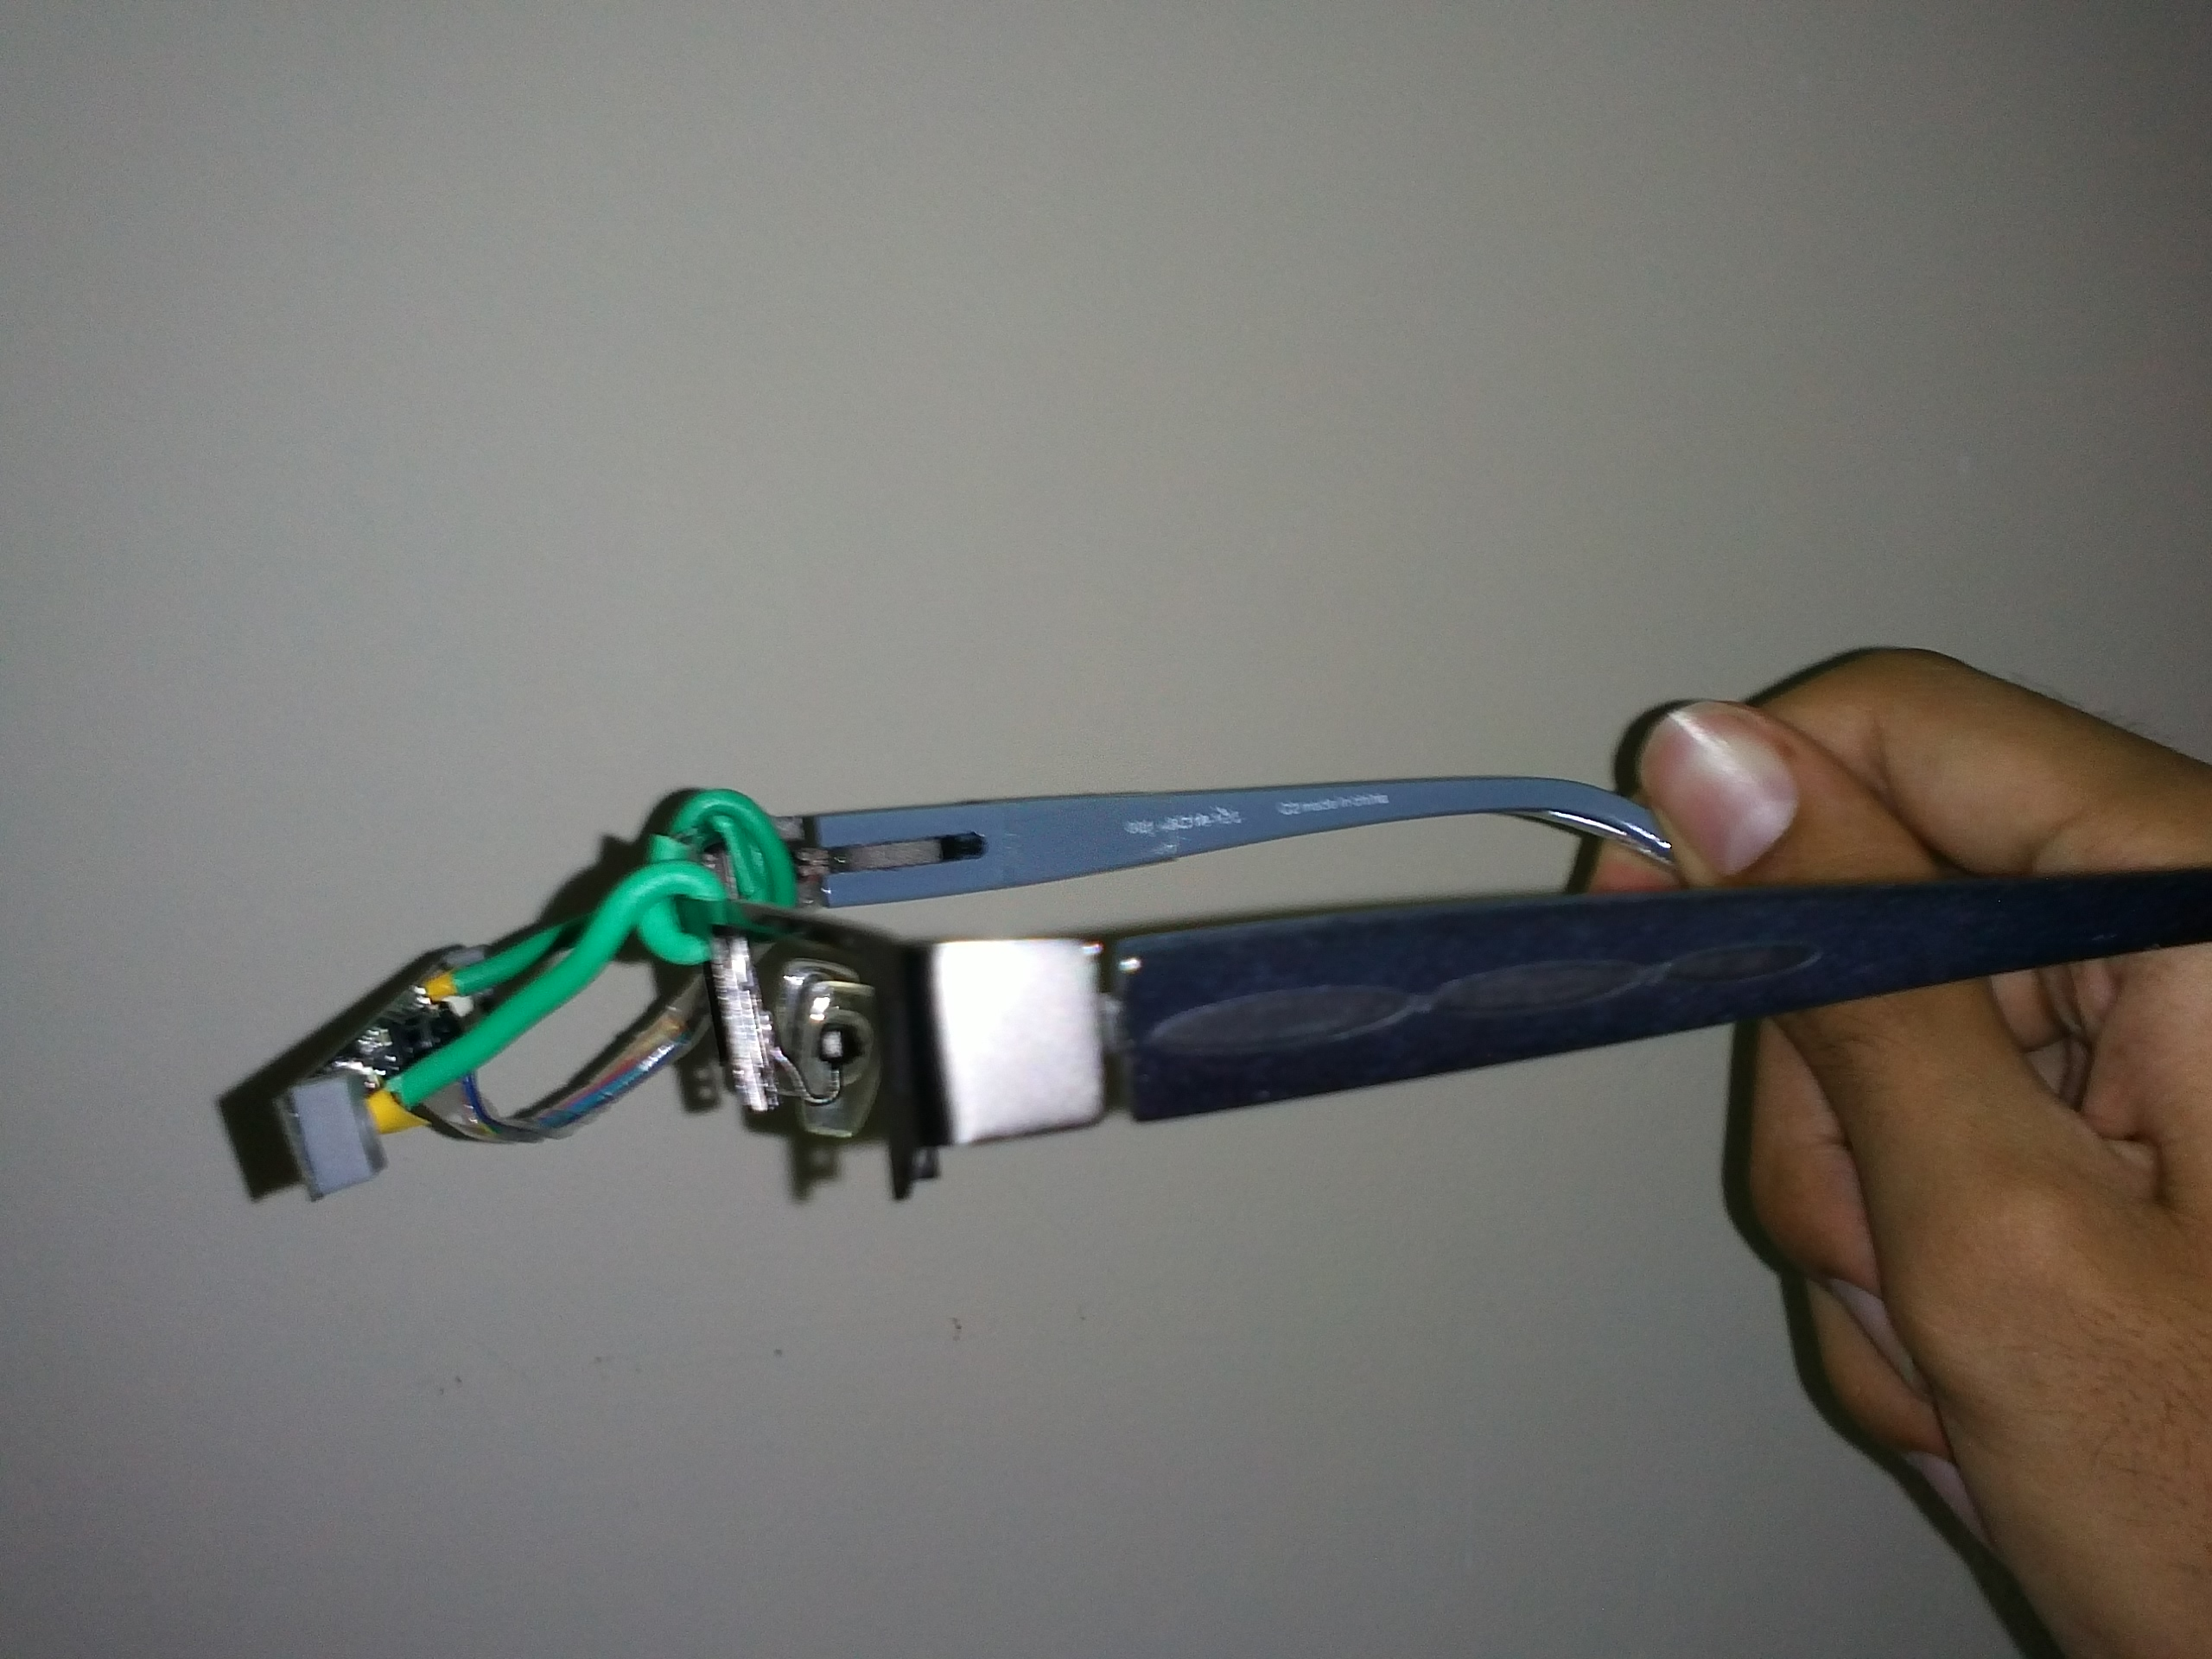
\includegraphics[width=.45\textwidth]{./Pictures/evaluation/cam_side_2.jpg}
	}
   \caption{Prototype of our cheap eye-tracking head set\label{fig:headset} }   
\end{dBox}   
\end{figure*}
